\documentclass[11pt]{article}
\usepackage[utf8]{inputenc}\usepackage[T1]{fontenc}\usepackage{lmodern}
\usepackage[margin=1in]{geometry}\usepackage{amsmath}\usepackage{booktabs}
\usepackage{graphicx}\usepackage[hidelinks]{hyperref}\usepackage{caption}\usepackage{float}
\captionsetup{justification=centering}
\graphicspath{{figures/}{figures_suppl/}}
\renewcommand{\thefigure}{S\arabic{figure}}
\renewcommand{\thetable}{S\arabic{table}}
\title{\bfseries Supplementary Material\\[2pt]
\large Does the choice of Sleep Regularity Index software change the conclusions?\\
A re-analysis of the NHANES 2011--2014 sleep-regularity--obesity association}
\author{Jürgen Degenfellner (ZHAW School of Health Sciences)}
\date{\today}
\begin{document}
\maketitle

This supplement reports, across the three SRI calculators (the original by-hand
Phillips implementation, \texttt{GGIR} and \texttt{sleepreg}), the same diagnostic
displays provided in the original study, plus the verification of the package
computations.

\section{Verification of the package computations}
On synthetic 7-day recordings with an analytically known SRI, all three
calculators returned the correct value (Table~\ref{tab:verify}); on a pseudo-random
pattern they agreed with the hand formula. This confirms the divergence reported in
the main text is a genuine consequence of algorithmic conventions, not an
implementation error.

\begin{table}[H]\centering
\caption{Synthetic verification (7 consecutive days, no missing epochs).}
\label{tab:verify}
\begin{tabular}{lcccc}
\toprule
Test case & expected & hand & \texttt{GGIR} & \texttt{sleepreg} \\
\midrule
7 identical days                 & $+100$ & $100.00$ & $100.00$ & $100.00$ \\
alternating pattern/complement   & $-100$ & $-100.00$ & $-100.00$ & $-100.00$ \\
agree on half the epochs         & $0$    & $0.00$ & $0.00$ & $-0.01$ \\
shifted pseudo-random            & ---    & $5.56$ & $5.89$ & $5.54$ \\
\bottomrule
\end{tabular}
\end{table}

\noindent\emph{Reproducibility note.} \texttt{sleepreg} (v1.3.5) aborts when a
recording starts exactly at local midnight (returning a missing value), and its
pinned dependency \texttt{GGIR}~2.0-0 prevents installation alongside current
\texttt{GGIR}; I therefore ran its SRI engine from source.

\section{Exact package invocations and parameter settings}
For full reproducibility I give the verbatim calls used to compute each SRI on
the byte-identical binary sleep/wake series, with package versions and every
argument (Table~\ref{tab:invoc}). The comparison uses each package's
\emph{default} settings throughout; the only non-defaults are output switches
(\texttt{wr.raster}, \texttt{overwr}) that do not affect the SRI value.
\texttt{sleepreg}'s SRI engine was run from its (\texttt{GGIR}-independent) source
functions, verbatim from v1.3.5, because its pinned dependency \texttt{GGIR}~2.0-0
cannot coexist with current \texttt{GGIR}; the synthetic verification above
confirms this reproduces the intended quantity.

\begin{verbatim}
# (1) Hand -- original Phillips formula, 1-min epochs, weekday-matched pairs
SRI = -100 + (200/N_valid) * sum( s[i] == s[i+1440] )   # over valid pairs

# (2) GGIR 3.3.6
df <- data.frame(time = as.POSIXct(ts, origin="1970-01-01", tz="UTC"),
                 sleepstate = as.numeric(s),
                 invalid    = as.integer(is.na(s)))
out <- GGIR::CalcSleepRegularityIndex(data=df, epochsize=60, desiredtz="UTC")
SRI <- mean(out$SleepRegularityIndex, na.rm=TRUE)  # mean over day-pairs

# (3) sleepreg 1.3.5 -- run from source, two-step pipeline
SWS_from_binarySW(binarySWdir=bindir, tsCol=2, binaryCol=1)
SRI_from_binary(binarydir=swsdir, col.trans=1, col.timestamp=2,
                wr.raster=FALSE, overwr=TRUE)
                # defaults kept: minSRIdays=5, exclNAhrs=6
\end{verbatim}

\begin{table}[H]\centering
\caption{Package versions and SRI-relevant parameter settings. All SRI-relevant
parameters are at package defaults; the non-default arguments (\texttt{wr.raster},
\texttt{overwr}) affect only the written output, not the SRI value.}
\label{tab:invoc}
\begin{tabular}{llp{8cm}}
\toprule
Calculator & Version & SRI-relevant settings (package defaults) \\
\midrule
Published (hand Phillips) & --- & 1-min epochs; day-of-week-matched consecutive day pairs \\
\texttt{GGIR}     & 3.3.6 & \texttt{epochsize=60} (1-min epochs); consecutive calendar-day pairs, time-of-day matched; mean over pairs \\
\texttt{sleepreg} & 1.3.5 & \texttt{minSRIdays=5}; \texttt{exclNAhrs=6}; 10-s epochs; continuous 24\,h lag \\
\bottomrule
\end{tabular}
\end{table}

\section{SRI distribution by calculator}
\begin{figure}[H]\centering
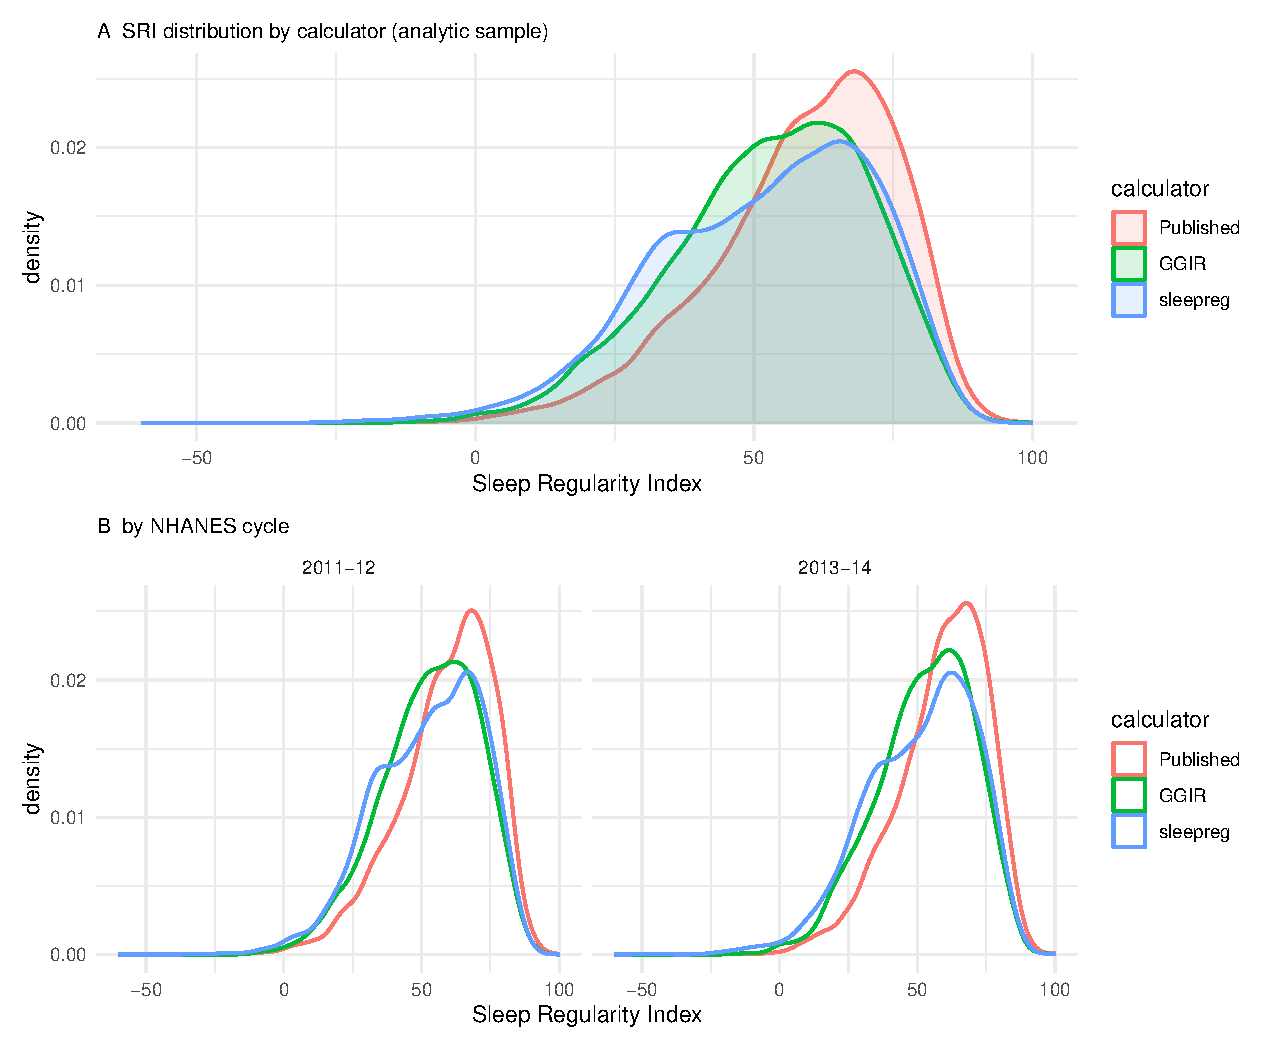
\includegraphics[width=0.95\textwidth]{S_SRI_distribution.pdf}
\caption{Distribution of the SRI by calculator on identical input: overall (A) and
by NHANES cycle (B). The package distributions are shifted lower than the
published SRI.}
\end{figure}

\section{Pairwise agreement (Bland--Altman)}
The all-versus-all pairwise agreement of the published SRI and the two packages
is shown in the main text (Figure~1); here I add the complementary Bland--Altman
view of each package against the published SRI.

\begin{figure}[H]\centering
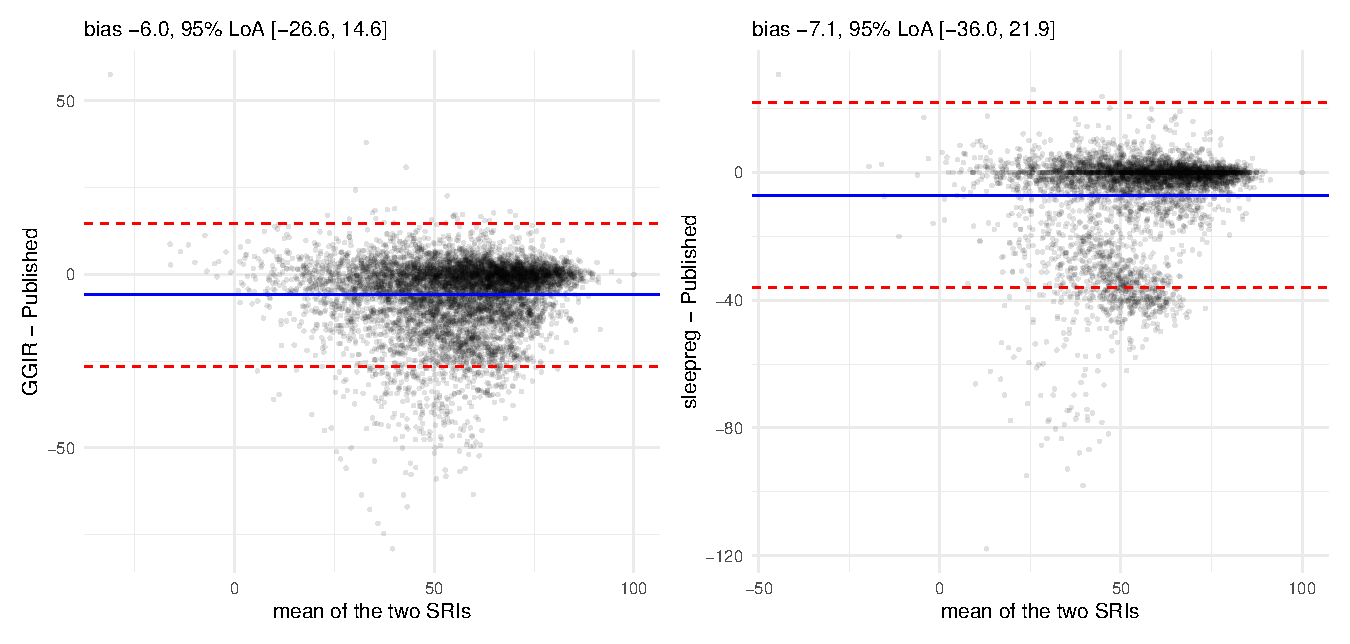
\includegraphics[width=\textwidth]{S_BlandAltman.pdf}
\caption{Bland--Altman agreement of each package SRI with the published SRI (blue:
mean difference; red dashed: 95\% limits of agreement).}
\end{figure}

\section{Structure of the disagreement}
\begin{figure}[H]\centering
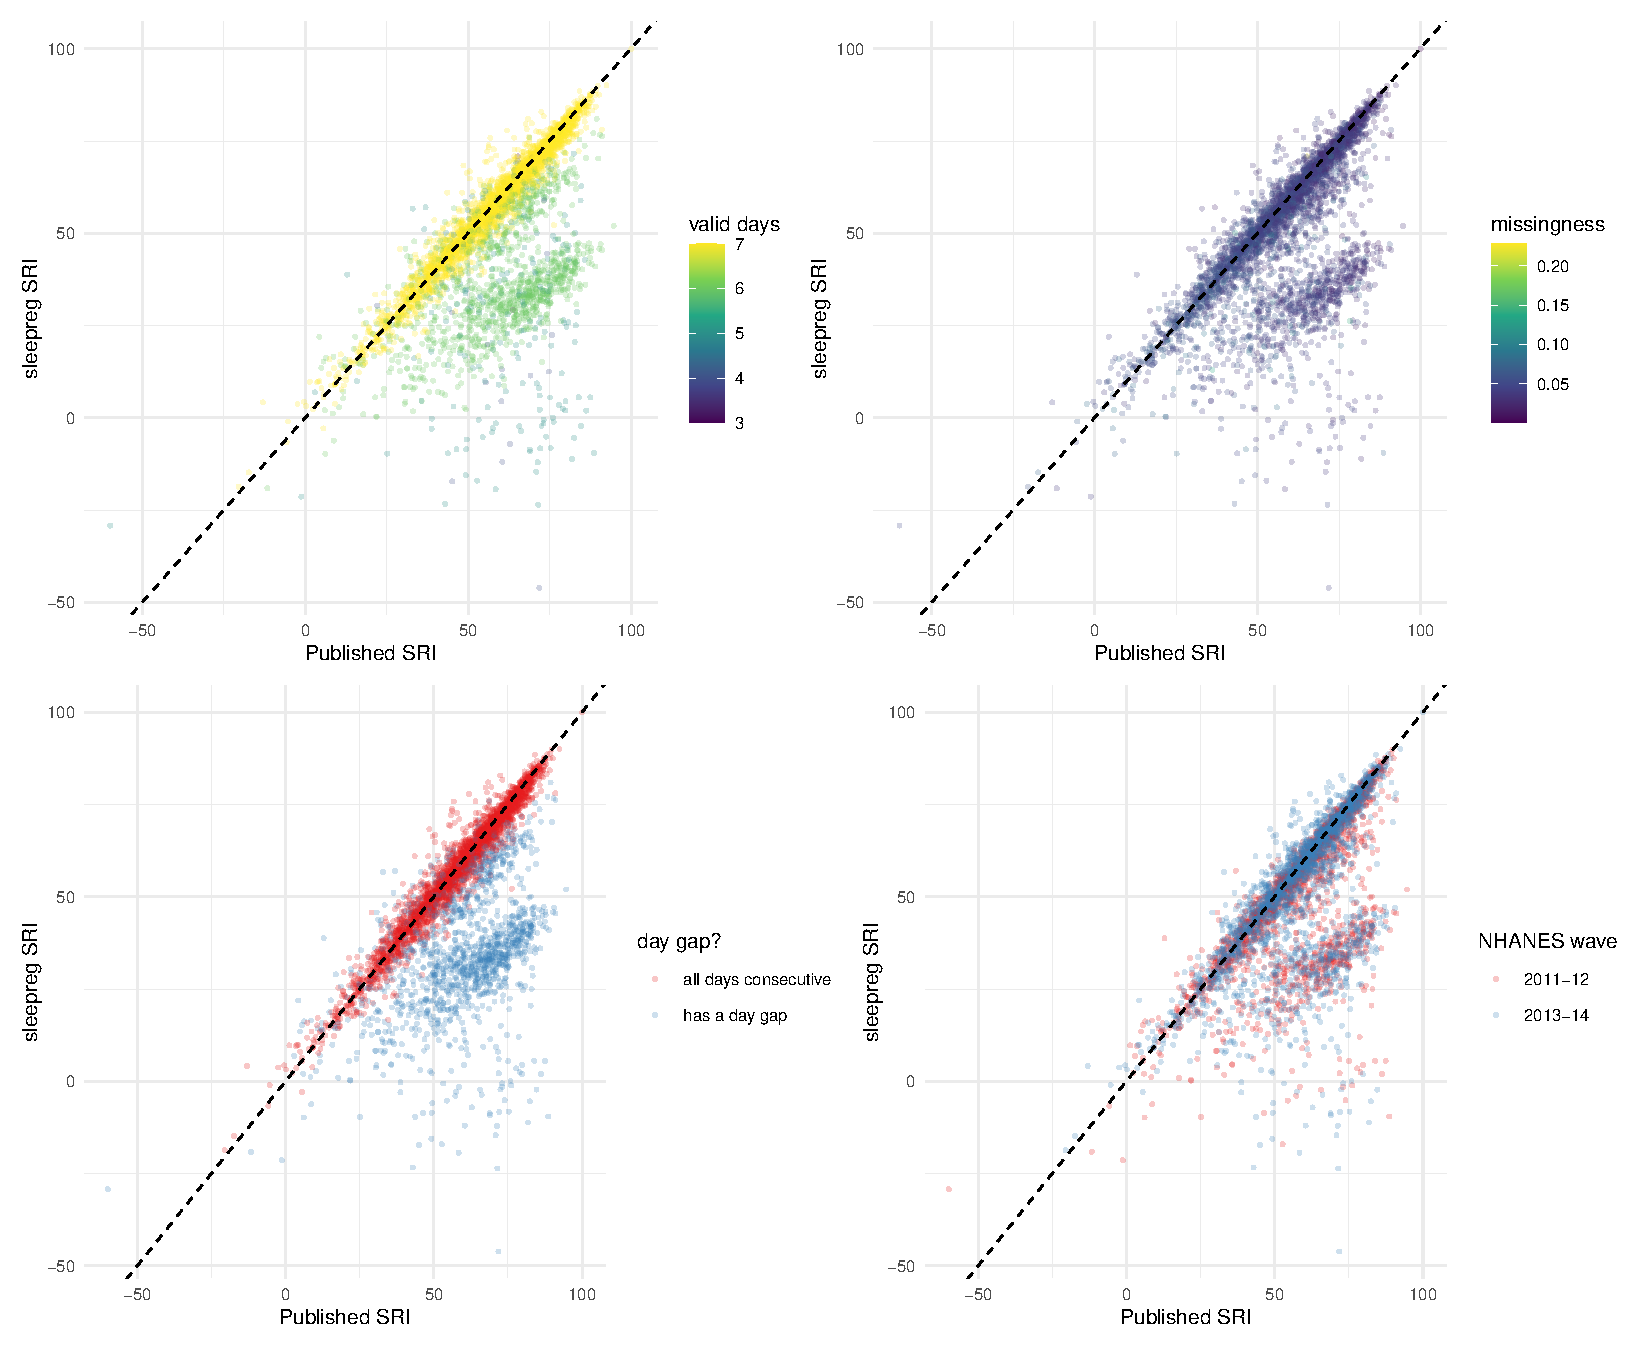
\includegraphics[width=\textwidth]{cloud_structure_Hand_vs_sleepreg.pdf}
\caption{The \texttt{sleepreg}-versus-published scatter coloured by candidate features.
The off-diagonal clouds track the number of valid (consecutive) days / the presence
of a day gap, not missingness or NHANES wave.}
\end{figure}

\section{The re-fitted model and predicted BMI by calculator}
Throughout this section ``the fully adjusted model'' is the fully adjusted,
non-interaction model of the original study, \textbf{Model~2 of Degenfellner
et~al.\ (2026), \emph{Journal of Biological Rhythms} 41(2):205--218, Table~3}:
$\log(\mathrm{BMI})$ regressed on the SRI plus age, sex, race/ethnicity,
education, household income, occupation category, alcohol consumption, smoking
status, vitamin~D, total caloric intake, PHQ-9 depression score, marital status
and physical activity, re-fitted with each SRI calculator substituted for the
exposure. The residual and assumption diagnostics for this model are shown per
calculator further below (\texttt{car::qqPlot()} and
\texttt{performance::check\_model()}).

\begin{figure}[H]\centering
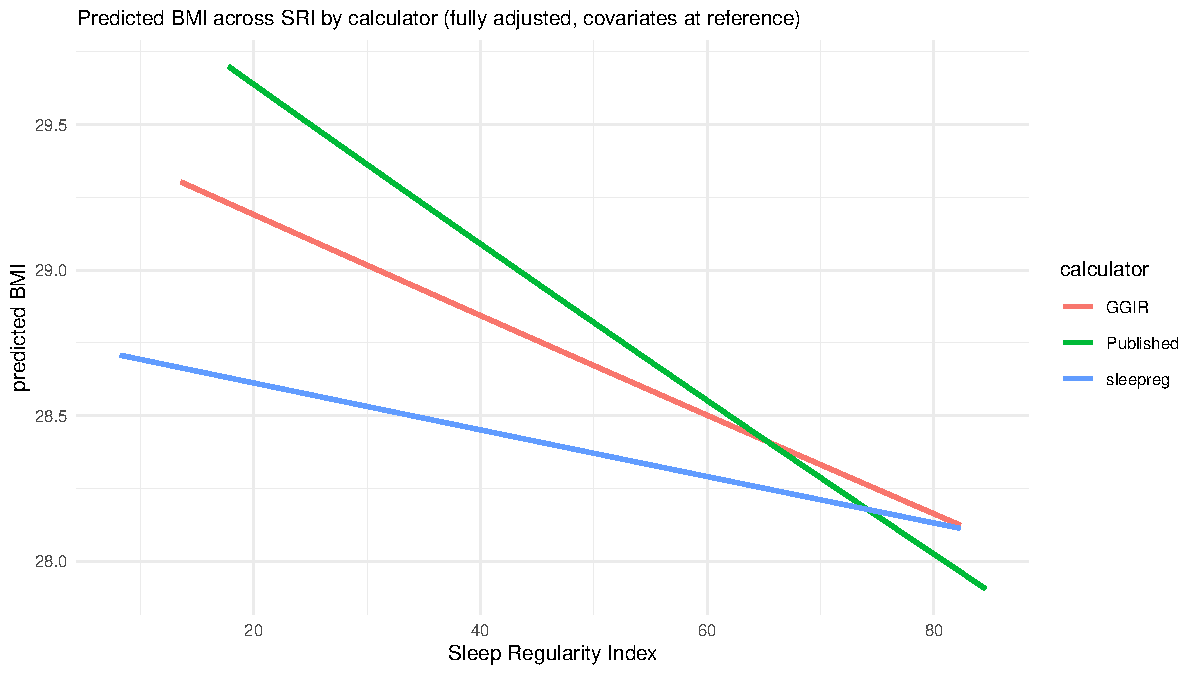
\includegraphics[width=0.85\textwidth]{S_predicted_BMI.pdf}
\caption{Predicted BMI across the SRI range under each calculator, from the fully
adjusted model (Model~2 of Degenfellner et~al.\ 2026, \emph{J Biol Rhythms}
41(2):205--218, Table~3; covariates at reference). The slope flattens from the
published SRI to \texttt{GGIR} to \texttt{sleepreg}.}
\end{figure}

\section{Are the re-fitted models well specified?}
I checked the assumptions of the fully adjusted model (Model~2 of Degenfellner
et~al.\ 2026, Table~3) re-fitted with each calculator (the per-calculator
\texttt{car::qqPlot()} and \texttt{check\_model()} panels below). The models are
\emph{equally well behaved across calculators}: adjusted $R^2\approx0.13$, residual
skewness $\approx0.31$ and excess kurtosis $\approx0.55$, and a maximum
variance-inflation factor of $2$ in every case. The corresponding \emph{magnitudes}
(mild right-skew of residuals, slight heteroscedasticity, a barely-curved SRI
term) are near-identical for all calculators and are already present in the
original model. In other words, the attenuation of the effect under
\texttt{GGIR}/\texttt{sleepreg} is not an artefact of those models fitting worse;
they fit essentially as well as the published one.

\section{\texttt{performance::check\_model()} and \texttt{car::qqPlot()} outputs}
For completeness, and matching the diagnostic displays of the original study, I
reproduce the full \texttt{performance::check\_model()} panel (posterior
predictive check, linearity, homogeneity of variance, influential observations,
collinearity, normality of residuals) for the fully adjusted model under each
calculator (Figs.~\ref{fig:cm_pub}--\ref{fig:cm_sr}), and the
\texttt{car::qqPlot()} of studentized residuals with 95\% envelopes
(Fig.~\ref{fig:qqcar}). The panels are visually indistinguishable across
calculators: the posterior predictive and homogeneity panels are well behaved,
all variance-inflation factors are below the conventional concern level, no
observation falls outside the influence contours, and the QQ panels show the same
mild heavy right tail in every case.

\begin{figure}[p]\centering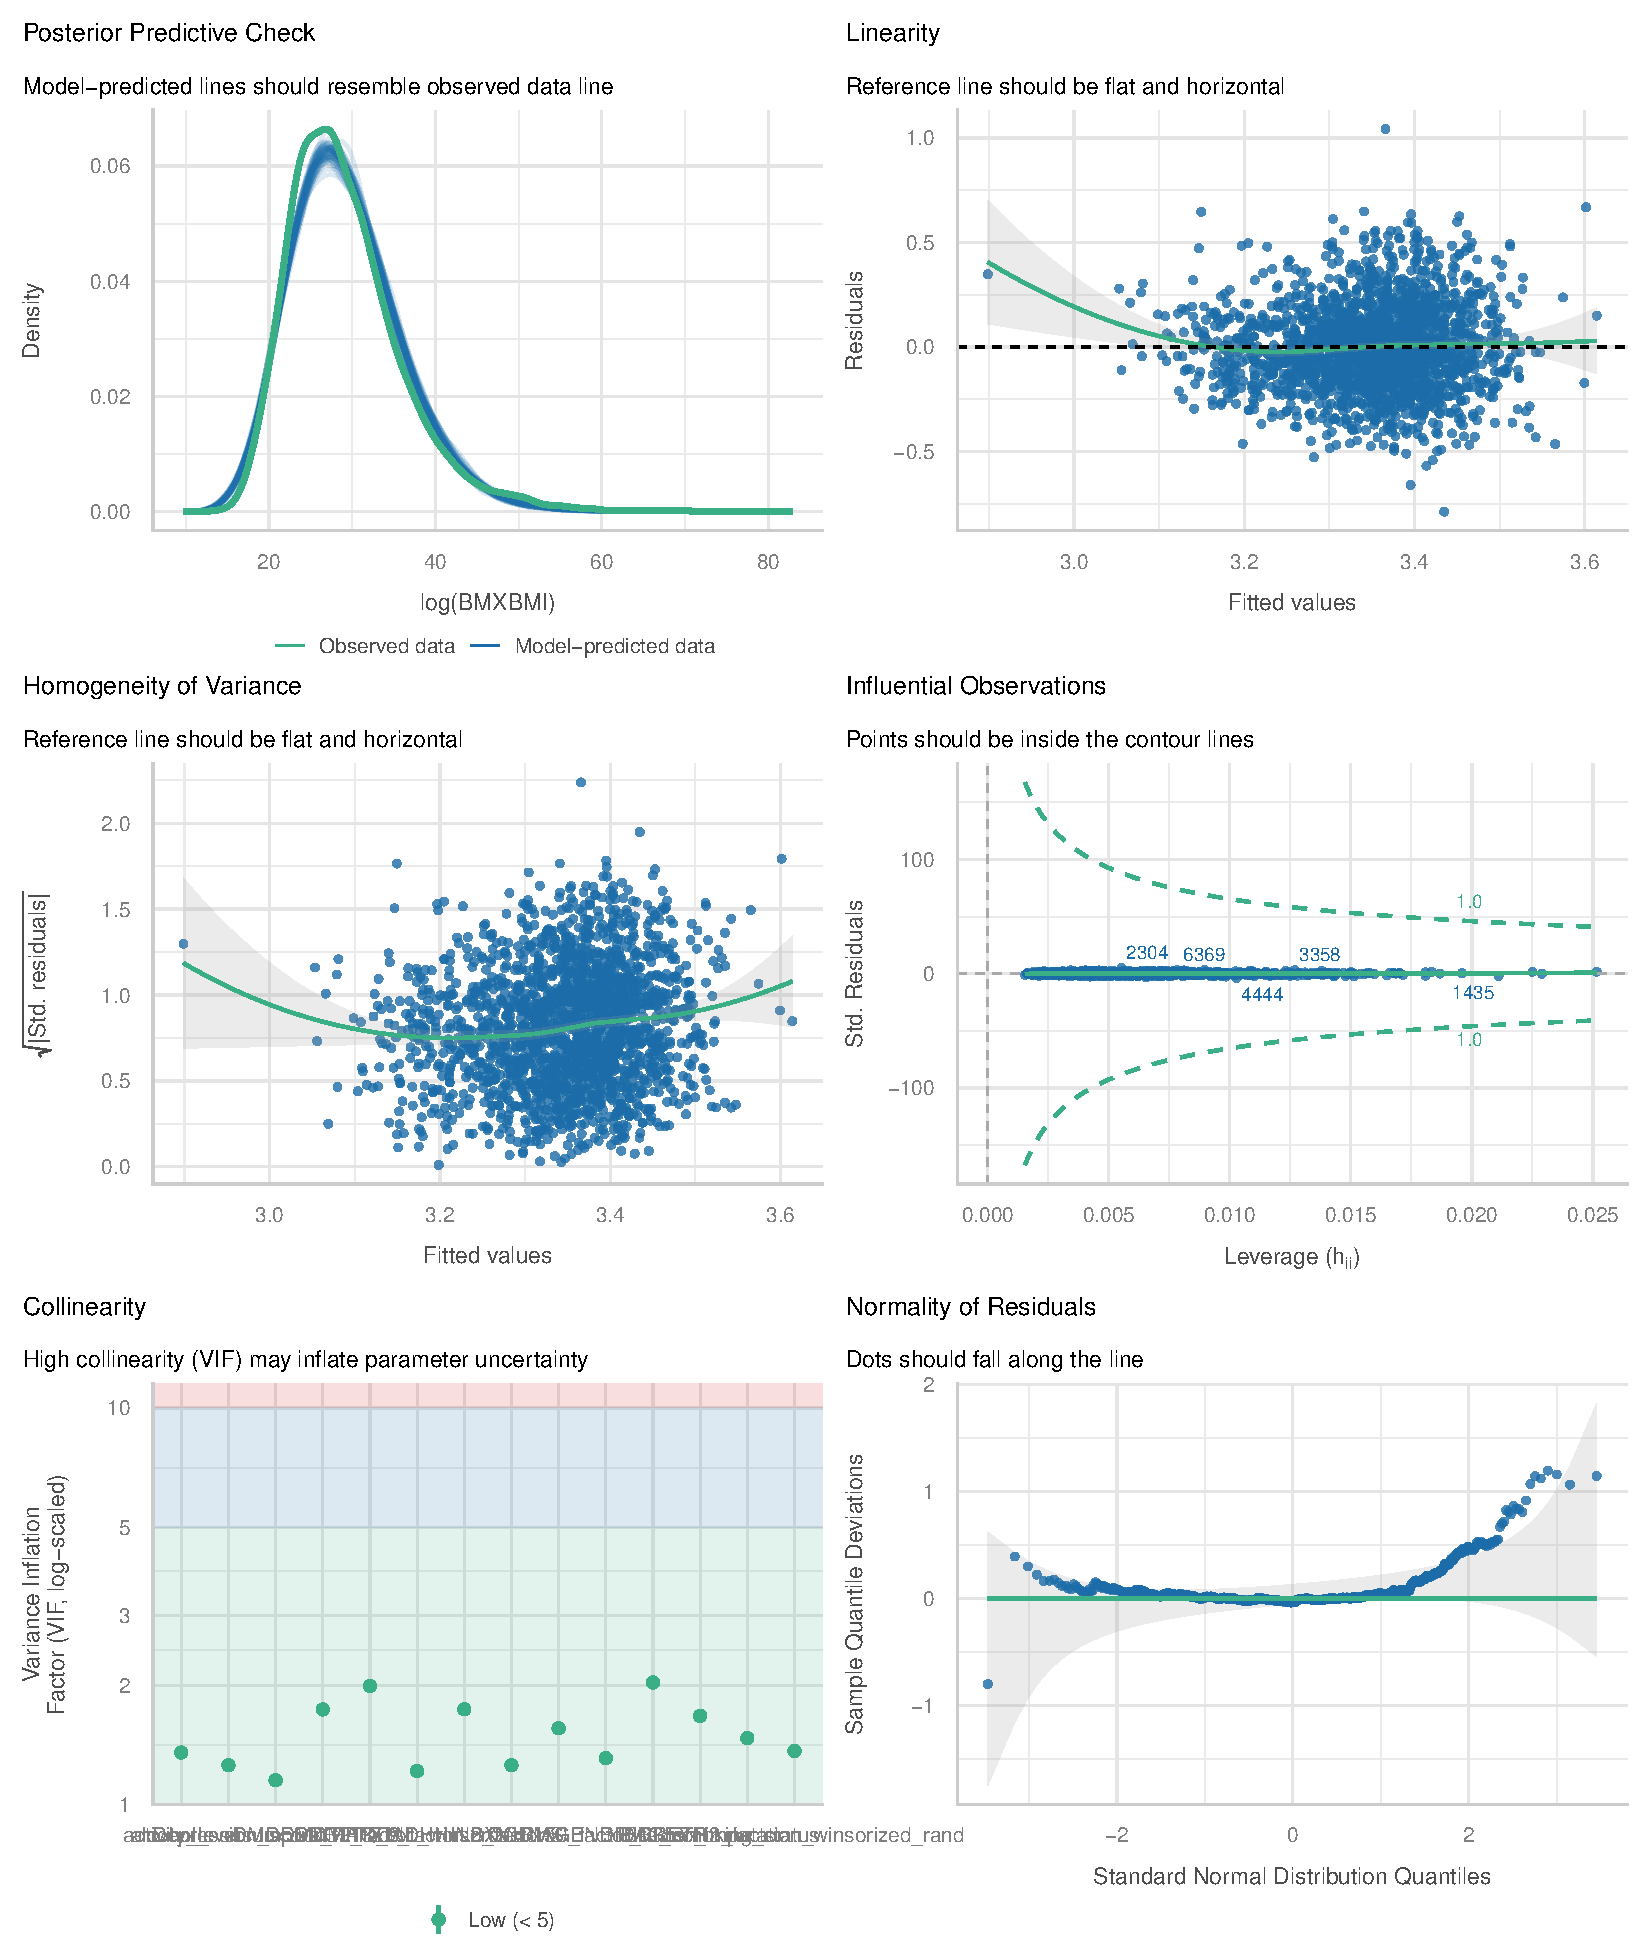
\includegraphics[width=\textwidth]{S_check_model_Published.pdf}
\caption{\texttt{check\_model()}: published SRI.}\label{fig:cm_pub}\end{figure}
\begin{figure}[p]\centering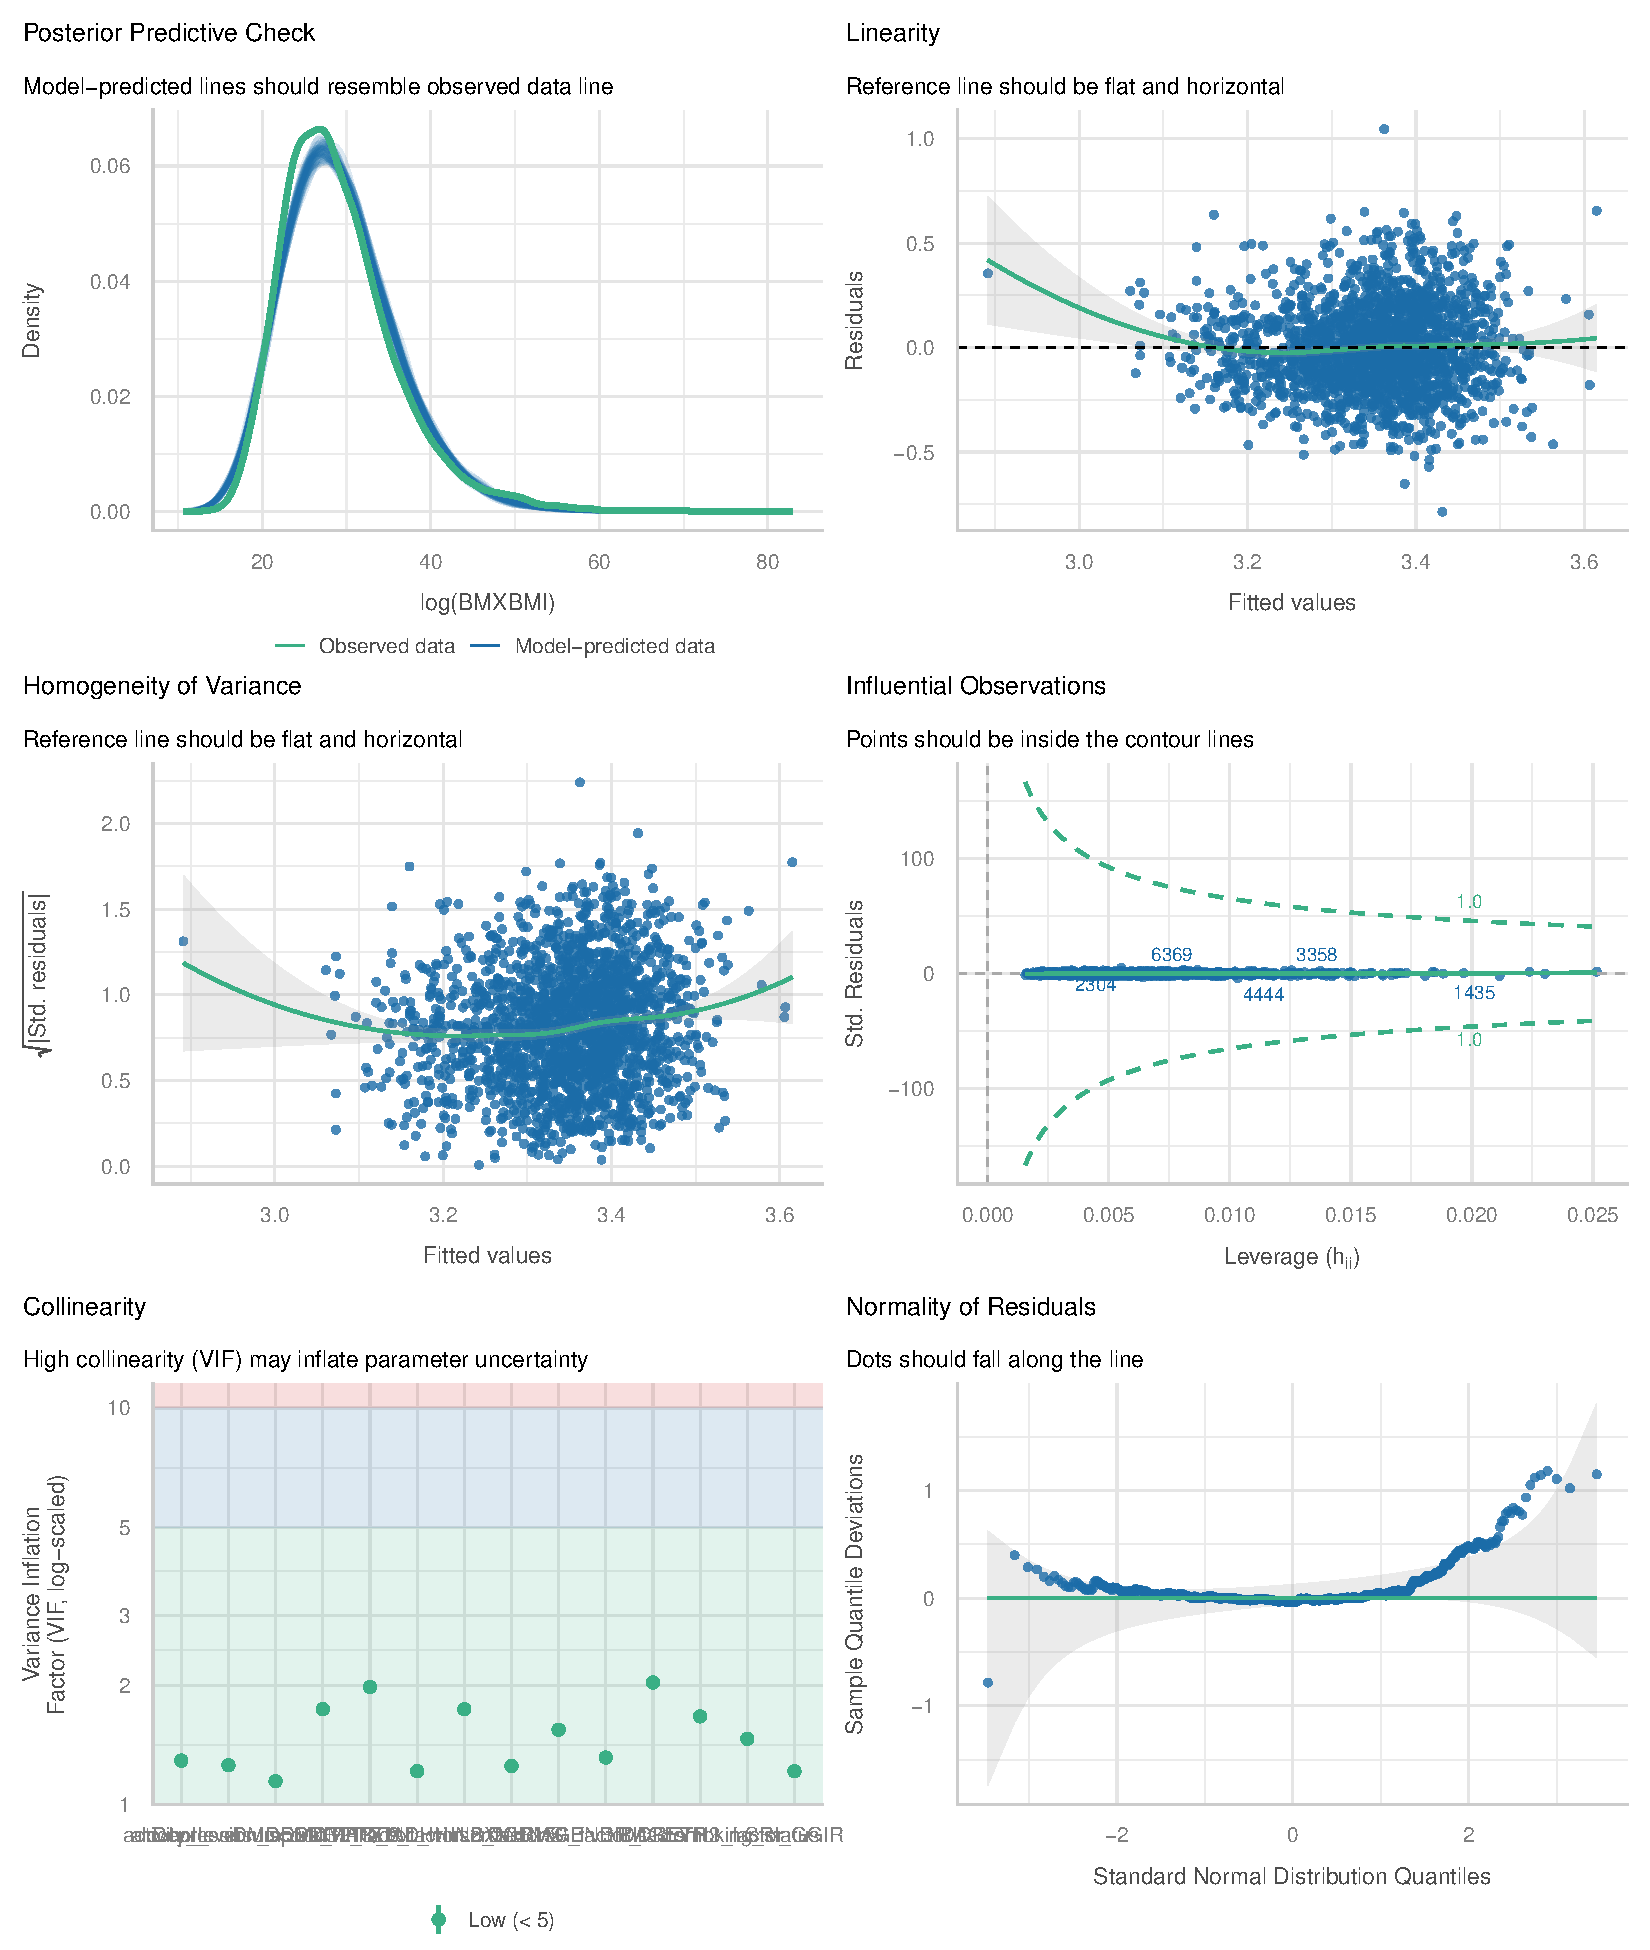
\includegraphics[width=\textwidth]{S_check_model_GGIR.pdf}
\caption{\texttt{check\_model()}: \texttt{GGIR} SRI.}\label{fig:cm_ggir}\end{figure}
\begin{figure}[p]\centering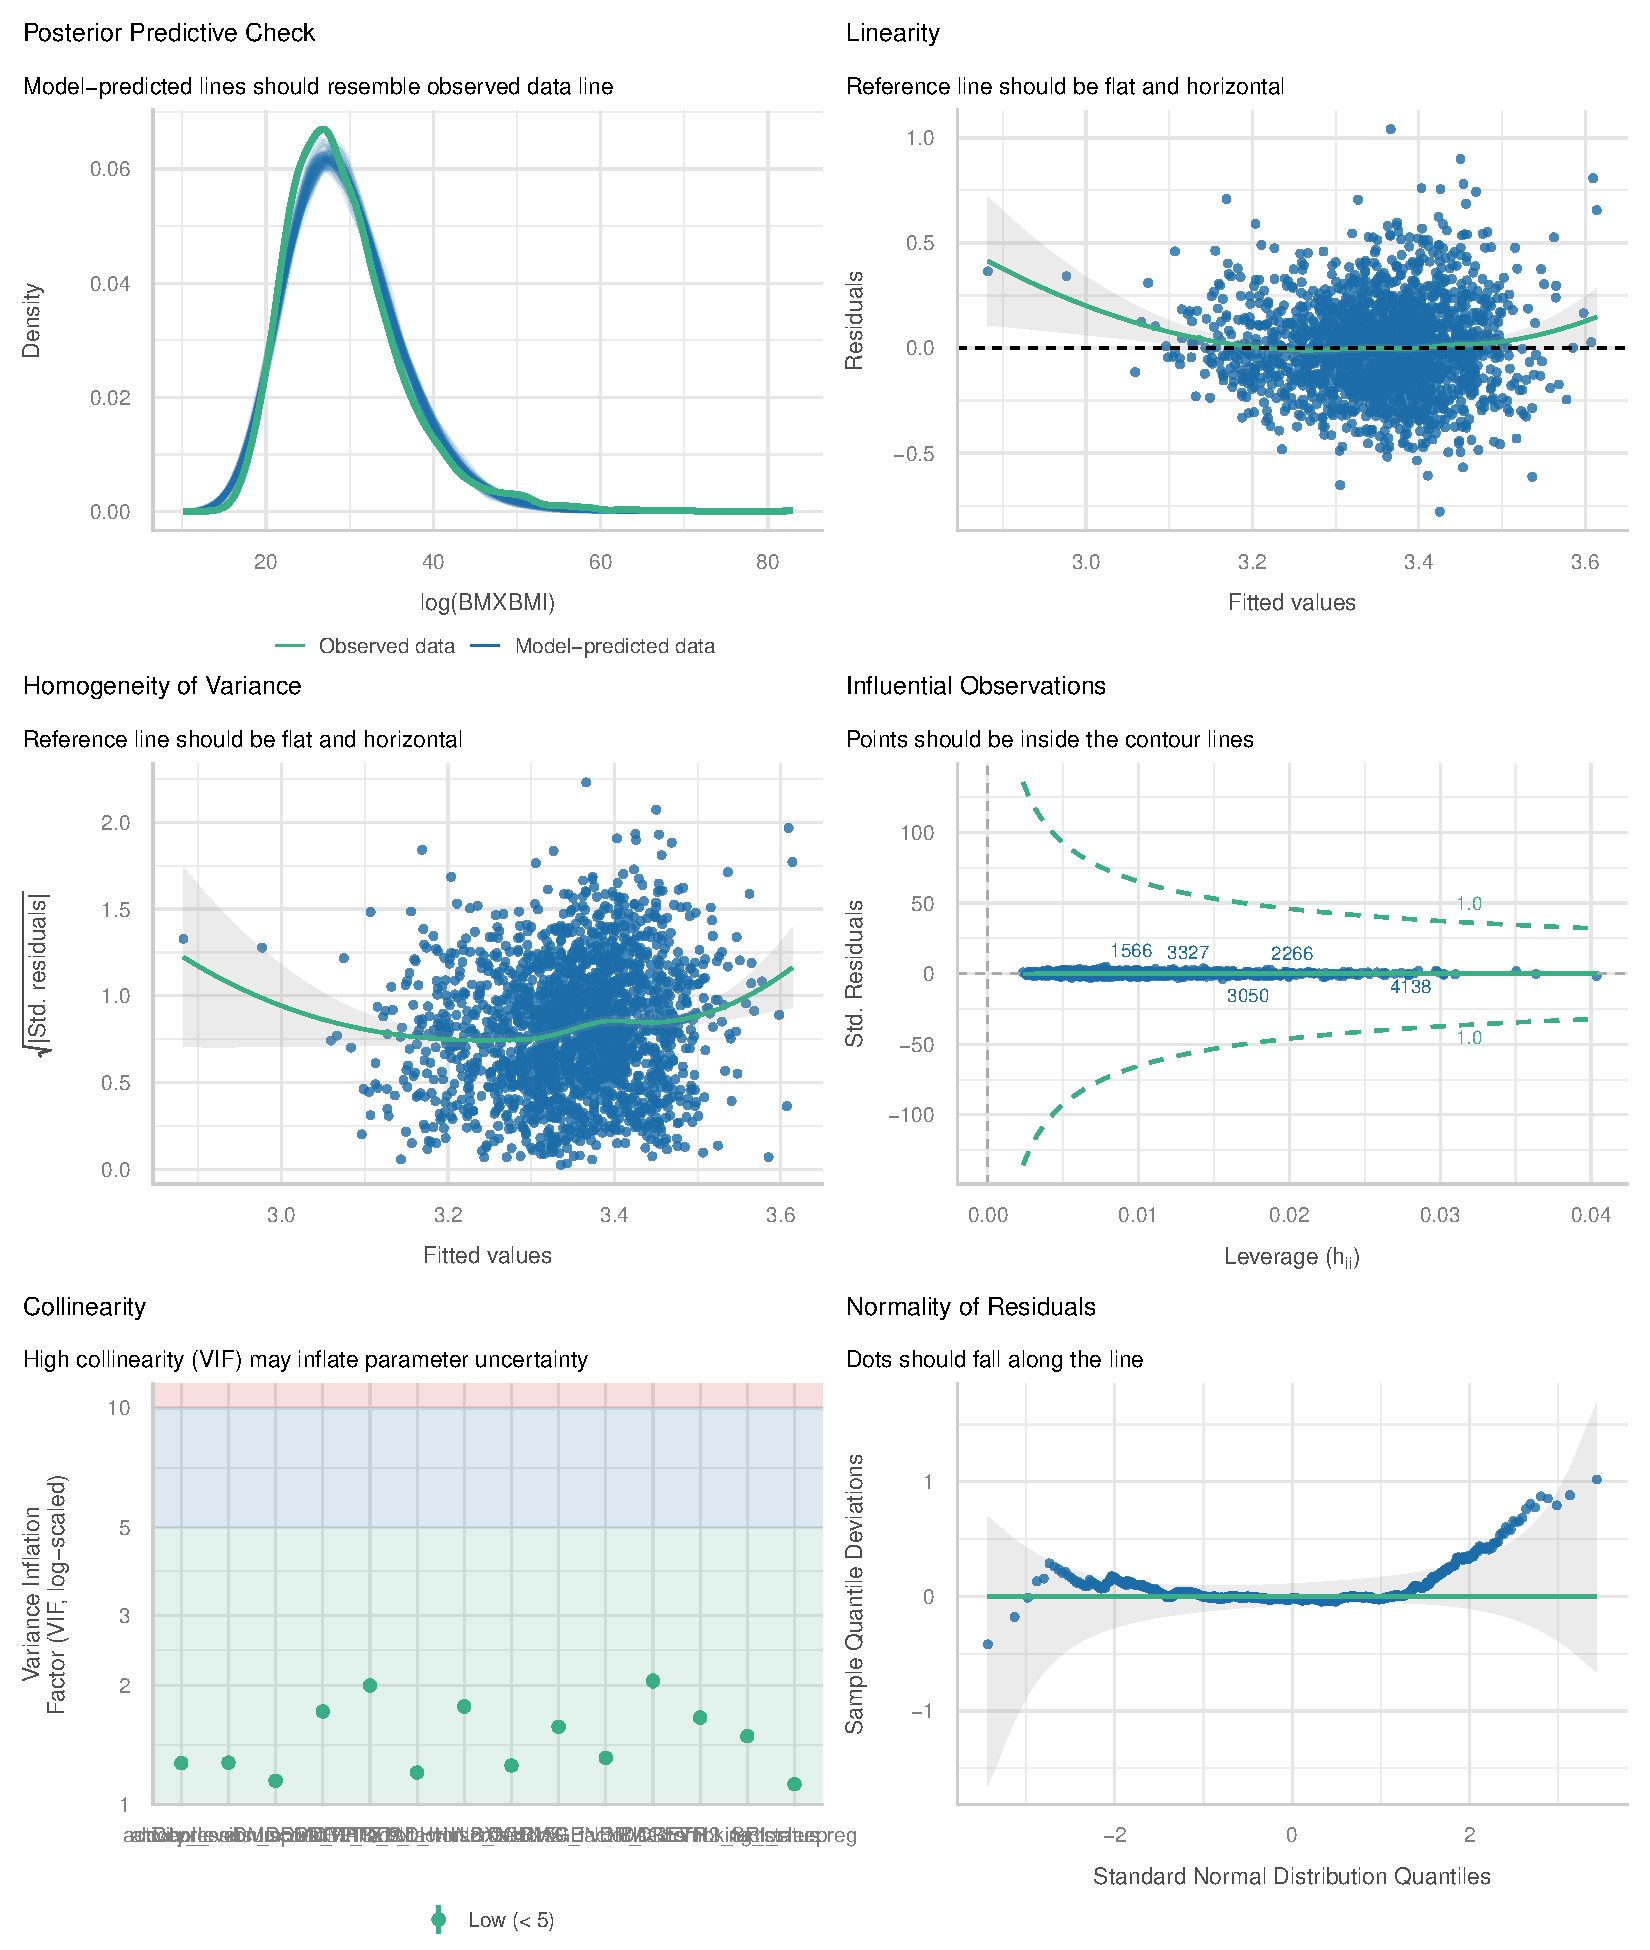
\includegraphics[width=\textwidth]{S_check_model_sleepreg.pdf}
\caption{\texttt{check\_model()}: \texttt{sleepreg} SRI.}\label{fig:cm_sr}\end{figure}

\begin{figure}[p]\centering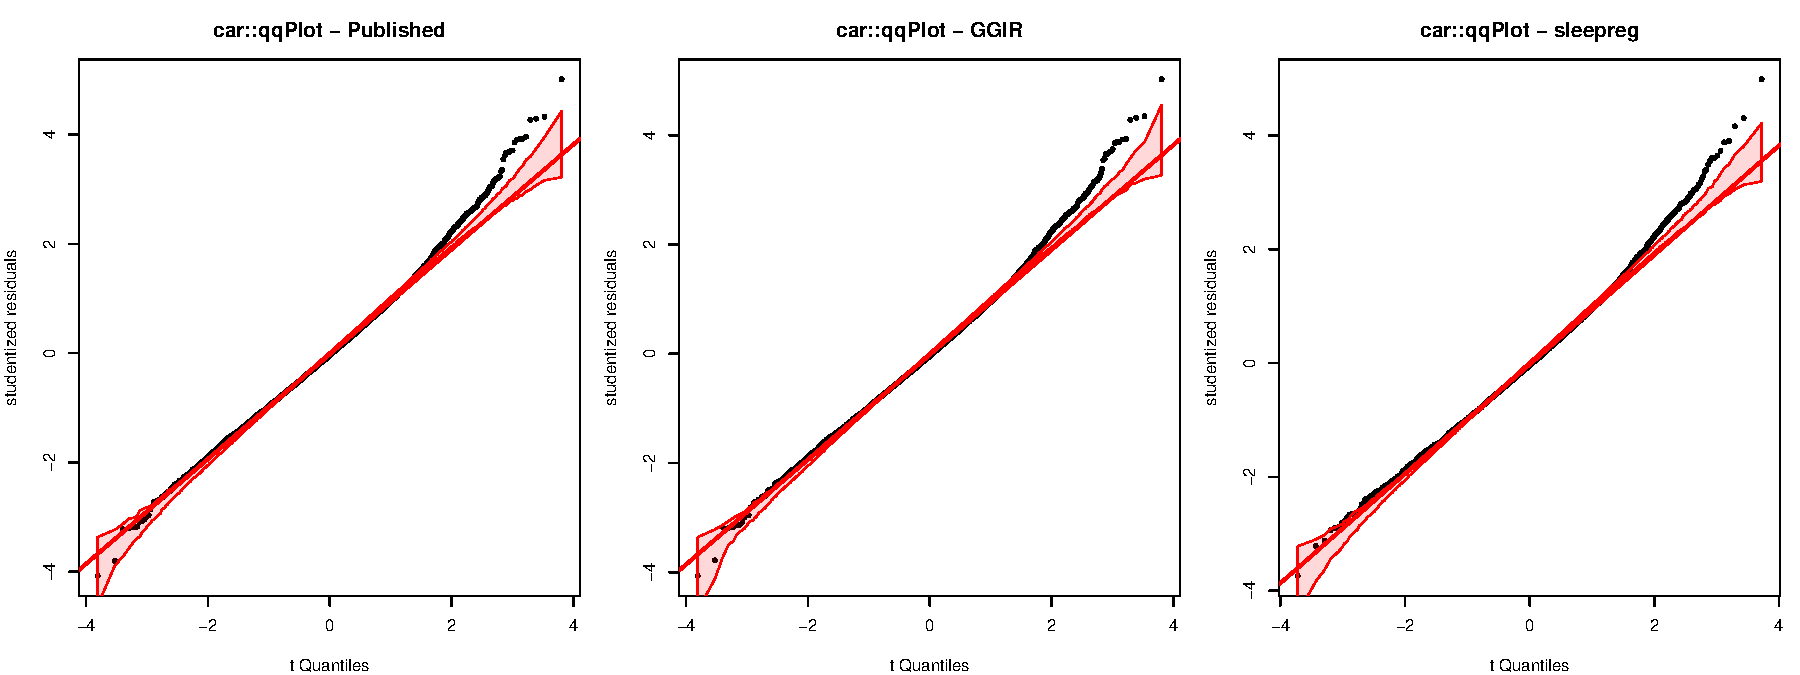
\includegraphics[width=0.9\textwidth]{S_qqPlot_car.pdf}
\caption{\texttt{car::qqPlot()} of studentized residuals with 95\% simulated
envelopes, fully adjusted model, by calculator. The same mild departure in the
upper tail appears for all three.}\label{fig:qqcar}\end{figure}

\end{document}
